
% ============================================================
%  DDR Memory Controller — Microarchitecture Deep-Dive
%  Beamer presentation  |  11 slides
%  Compile:  pdflatex -shell-escape DDR_MC_Presentation.tex
%            (run twice for cross-refs)
% ============================================================
\documentclass[aspectratio=169,10pt]{beamer}

% ── Packages ────────────────────────────────────────────────────────────────
\usepackage{tikz}
\usetikzlibrary{arrows.meta, fit, backgrounds, calc, positioning, matrix}
\usepackage{xcolor}
\usepackage[T1]{fontenc}
\usepackage{lmodern}
\usepackage{amsmath}
\usepackage{booktabs}
\usepackage{colortbl}
\usepackage{array}
\usepackage{microtype}
\usepackage{hyperref}
\usepackage{graphicx}

% ── Palette ─────────────────────────────────────────────────────────────────
\definecolor{Navy}   {HTML}{0D1B2A}
\definecolor{Teal}   {HTML}{1A6060}
\definecolor{TealF}  {HTML}{D4EEEE}
\definecolor{Blue}   {HTML}{1A3A7A}
\definecolor{BlueF}  {HTML}{DDE3F5}
\definecolor{Amber}  {HTML}{7A4010}
\definecolor{AmberF} {HTML}{FAE8D4}
\definecolor{Purp}   {HTML}{534AB7}
\definecolor{PurpF}  {HTML}{EEEDFE}
\definecolor{Green}  {HTML}{3B6D11}
\definecolor{GreenF} {HTML}{EAF3DE}
\definecolor{MGray}  {HTML}{5F5E5A}
\definecolor{LGray}  {HTML}{E8EBF0}
\definecolor{BypassR}{HTML}{993C1D}
\definecolor{ddr3col}{HTML}{1A5276}
\definecolor{ddr4col}{HTML}{1A7A4A}
\definecolor{ddr5col}{HTML}{6E2B8C}

% ── Beamer theme ────────────────────────────────────────────────────────────
\usetheme{default}
\usecolortheme{default}
\setbeamertemplate{navigation symbols}{}
\setbeamertemplate{frametitle}{%
  \begin{beamercolorbox}[wd=\paperwidth,ht=0.72cm,dp=0pt,leftskip=0.35cm]{frametitle}%
    \vbox to 0.72cm{\vfil
      \usebeamerfont{frametitle}\insertframetitle
      \ifx\insertframesubtitle\@empty\else
        \hfill{\footnotesize\color{cyan!60!white}\insertframesubtitle}%
      \fi
    \hspace*{0.35cm}\vfil}%
  \end{beamercolorbox}%
}
\setbeamercolor{frametitle}{bg=Navy, fg=white}
\setbeamerfont{frametitle}{size=\large,series=\bfseries}
\setbeamercolor{background canvas}{bg=LGray!30!white}
\setbeamercolor{normal text}{fg=Navy}
\setbeamertemplate{footline}{%
  \hfill{\tiny\color{MGray}\insertframenumber/\inserttotalframenumber\hspace*{4pt}}%
  \vspace*{3pt}%
}

% ── TikZ block styles ────────────────────────────────────────────────────────
\tikzset{
  blk/.style args={#1/#2}{
    rectangle, rounded corners=4pt,
    draw=#1, fill=#2, text=#1,
    font=\scriptsize\bfseries, align=center,
    inner sep=5pt, minimum width=2.0cm, minimum height=0.75cm,
    line width=0.8pt,
  },
  sblk/.style args={#1/#2}{
    rectangle, rounded corners=3pt,
    draw=#1, fill=#2, text=#1,
    font=\tiny\bfseries, align=center,
    inner sep=3pt, minimum width=1.6cm, minimum height=0.6cm,
    line width=0.7pt,
  },
  rgn/.style args={#1}{
    draw=#1, fill=#1!6, rounded corners=6pt,
    dashed, line width=0.9pt,
  },
  arr/.style args={#1}{
    -{Stealth[length=4pt,width=3pt]},
    line width=0.8pt, color=#1,
  },
  lbl/.style={
    font=\tiny\itshape, text=MGray,
    fill=white, inner sep=1pt,
  },
  % image placeholder box
  imgbox/.style={
    rectangle, rounded corners=3pt,
    draw=MGray!50, fill=LGray,
    dashed, line width=0.6pt,
    font=\tiny\itshape, text=MGray, align=center,
    inner sep=5pt,
  },
}

% ── Reusable image placeholder ───────────────────────────────────────────────
% Usage: \imgplaceholder{width}{height}{filename}
\newcommand{\imgplaceholder}[3]{%
  \begin{tikzpicture}
    \node[imgbox, minimum width=#1, minimum height=#2]
      {[IMAGE: \texttt{#3}]};
  \end{tikzpicture}%
}

% ── Info card helper ─────────────────────────────────────────────────────────
\newcommand{\infocard}[3]{%
  \begin{tikzpicture}
    \node[rectangle, rounded corners=4pt,
          draw=#1, fill=#2, text=Navy,
          inner sep=7pt, line width=0.9pt,
          text width=\linewidth-14pt-2\pgflinewidth] {#3};
  \end{tikzpicture}%
}

% ============================================================
\begin{document}

% ── Slide 1: Title ───────────────────────────────────────────────────────────
\setbeamercolor{background canvas}{bg=Navy}
\begin{frame}[plain]
  \vspace*{0.5cm}
  \begin{center}
    {\huge\bfseries\color{white}Reconfigurable Universal DDR Memory Controller}\\[6pt]
    {\large\color{cyan!70!white}Microarchitecture Deep-Dive}\\[4pt]
    {\small\color{blue!40!white}DDR2 · DDR3 · DDR4 · DDR5 \quad|\quad AXI4 Host Interface \quad|\quad DFI PHY}
  \end{center}

  \vspace*{0.25cm}
  {\color{Navy!40!white}\rule{\linewidth}{0.4pt}}
  \vspace*{0.15cm}

  \begin{center}
  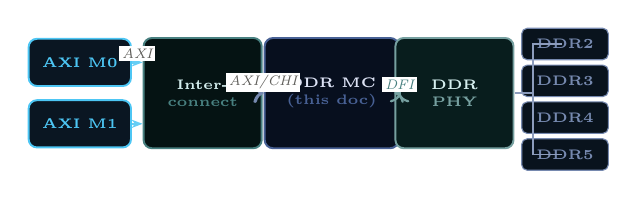
\begin{tikzpicture}[x=1cm,y=1cm,scale=0.78]
    \node[sblk=cyan!70!white/Navy!80!black,
          minimum width=1.3cm, minimum height=0.6cm] (m0) at (0, 0.6)
          {\color{cyan!70!white}AXI M0};
    \node[sblk=cyan!70!white/Navy!80!black,
          minimum width=1.3cm, minimum height=0.6cm] (m1) at (0,-0.4)
          {\color{cyan!70!white}AXI M1};
    \node[sblk=Teal!80!white/Teal!20!black,
          minimum width=1.5cm, minimum height=1.4cm] (ic) at (2.0, 0.1)
          {\color{TealF}Inter-\\connect};
    \node[sblk=Blue!80!white/Blue!25!black,
          minimum width=1.7cm, minimum height=1.4cm] (mc) at (4.1, 0.1)
          {\color{BlueF}DDR MC\\(this doc)};
    \node[sblk=Teal!60!white/Teal!30!black,
          minimum width=1.5cm, minimum height=1.4cm] (phy) at (6.1, 0.1)
          {\color{TealF}DDR\\PHY};
    \foreach \lbl/\yi/\c in {
        DDR2/0.9/Blue!60!white,
        DDR3/0.3/Blue!60!white,
        DDR4/-0.3/Blue!60!white,
        DDR5/-0.9/Blue!60!white}{
      \node[rectangle, rounded corners=2pt,
            draw=\c, fill=Navy!70!black,
            font=\tiny\bfseries, text=\c,
            minimum width=1.1cm, minimum height=0.4cm,
            inner sep=2pt] at (7.9,\yi) {\lbl};
    }
    \draw[arr=cyan!60!white] (m0.east) -- node[above,lbl]{\tiny AXI}
        (m0.east -| ic.west);
    \draw[arr=cyan!60!white] (m1.east) -- (m1.east -| ic.west);
    \draw[arr=Blue!60!white,<->] (ic.east) --
        node[above,lbl]{\tiny AXI/CHI} (mc.west);
    \draw[arr=Teal!60!white,<->] (mc.east) --
        node[above,lbl]{\tiny\color{Teal!80!white}DFI} (phy.east -| mc.east)
        -- (phy.west);
    \draw[Blue!50!white, line width=0.6pt] (phy.east) -- ++(0.3,0)
        |- (7.85, 0.9);
    \draw[Blue!50!white, line width=0.6pt] ($(phy.east)+(0.3,0)$)
        |- (7.85,-0.9);
  \end{tikzpicture}
  \end{center}

  \vspace*{0.1cm}
  \begin{center}
    {\tiny\color{blue!40!white}System-level context — MC block is the scope of this document}
  \end{center}
\end{frame}
\setbeamercolor{background canvas}{bg=LGray!30!white}

% ── Slide 2: Recap ───────────────────────────────────────────────────────────
\begin{frame}{Recap — Previous Meeting}
              {DFI · AXI4 · PHY Interface}
  \vspace*{0.05cm}
  \begin{columns}[T,totalwidth=\linewidth]
    \begin{column}{0.49\linewidth}
      \infocard{Blue}{BlueF}{%
        {\small\bfseries\color{Blue}AXI4 Host Interface}\\[3pt]
        \scriptsize
        \textbullet\ INCR bursts only — WRAP/FIXED not used\\[2pt]
        \textbullet\ 64-bit data bus; outstanding multi-ID supported\\[2pt]
        \textbullet\ No narrow/unaligned/exclusive transfers\\[2pt]
        \textbullet\ Read responses ordered per AXID via ROB
      }

      \vspace*{5pt}
      \infocard{Amber}{AmberF}{%
        {\small\bfseries\color{Amber}DDR PHY}\\[3pt]
        \scriptsize
        \textbullet\ Handles IO calibration, DQS alignment, ODT, ZQ cal\\[2pt]
        \textbullet\ Decouples MC from generation-specific electrical signalling\\[2pt]
        \textbullet\ Same DFI signals work for DDR3/DDR4/DDR5/LPDDR4\\[2pt]
        \textbullet\ Upstream boundary for this project scope
      }
    \end{column}

    \begin{column}{0.49\linewidth}
      \infocard{Teal}{TealF}{%
        {\small\bfseries\color{Teal}DFI (DDR PHY Interface)}\\[3pt]
        \scriptsize
        \textbullet\ Standard MC\,$\leftrightarrow$\,PHY contract — MC never drives DDR pins\\[2pt]
        \textbullet\ DFI 5.2: unified cmd bus, per-byte DQ/DQS lanes\\[2pt]
        \textbullet\ MC drives \texttt{dfi\_address}, \texttt{dfi\_cs\_n}, \texttt{dfi\_we\_n}, \texttt{dfi\_cas\_n}\\[2pt]
        \textbullet\ Write/read latency signalled via \texttt{dfi\_wrdata\_en}
      }

      \vspace*{5pt}
      \infocard{Purp}{PurpF}{%
        {\small\bfseries\color{Purp}Config Register File}\\[3pt]
        \scriptsize
        \textbullet\ All timing params at boot: tRCD, tRAS, tRP, tRFC, tFAW\ldots\\[2pt]
        \textbullet\ Addr-mapping mode, burst length, page policy per-rank\\[2pt]
        \textbullet\ Same RTL correct across all supported DDR generations\\[2pt]
        \textbullet\ Init FSM reads command sequence from reg file
      }
    \end{column}
  \end{columns}

  \vspace*{4pt}
  {\scriptsize\itshape\color{MGray}All concepts above feed directly into the MC
   microarchitecture discussed today.}
\end{frame}

% ── Slide 3: High-Level Microarchitecture ────────────────────────────────────
\begin{frame}{High-Level Microarchitecture}
              {Three-Domain Pipeline}
  \vspace*{-0.15cm}
  \begin{center}
  \scalebox{0.62}{%
  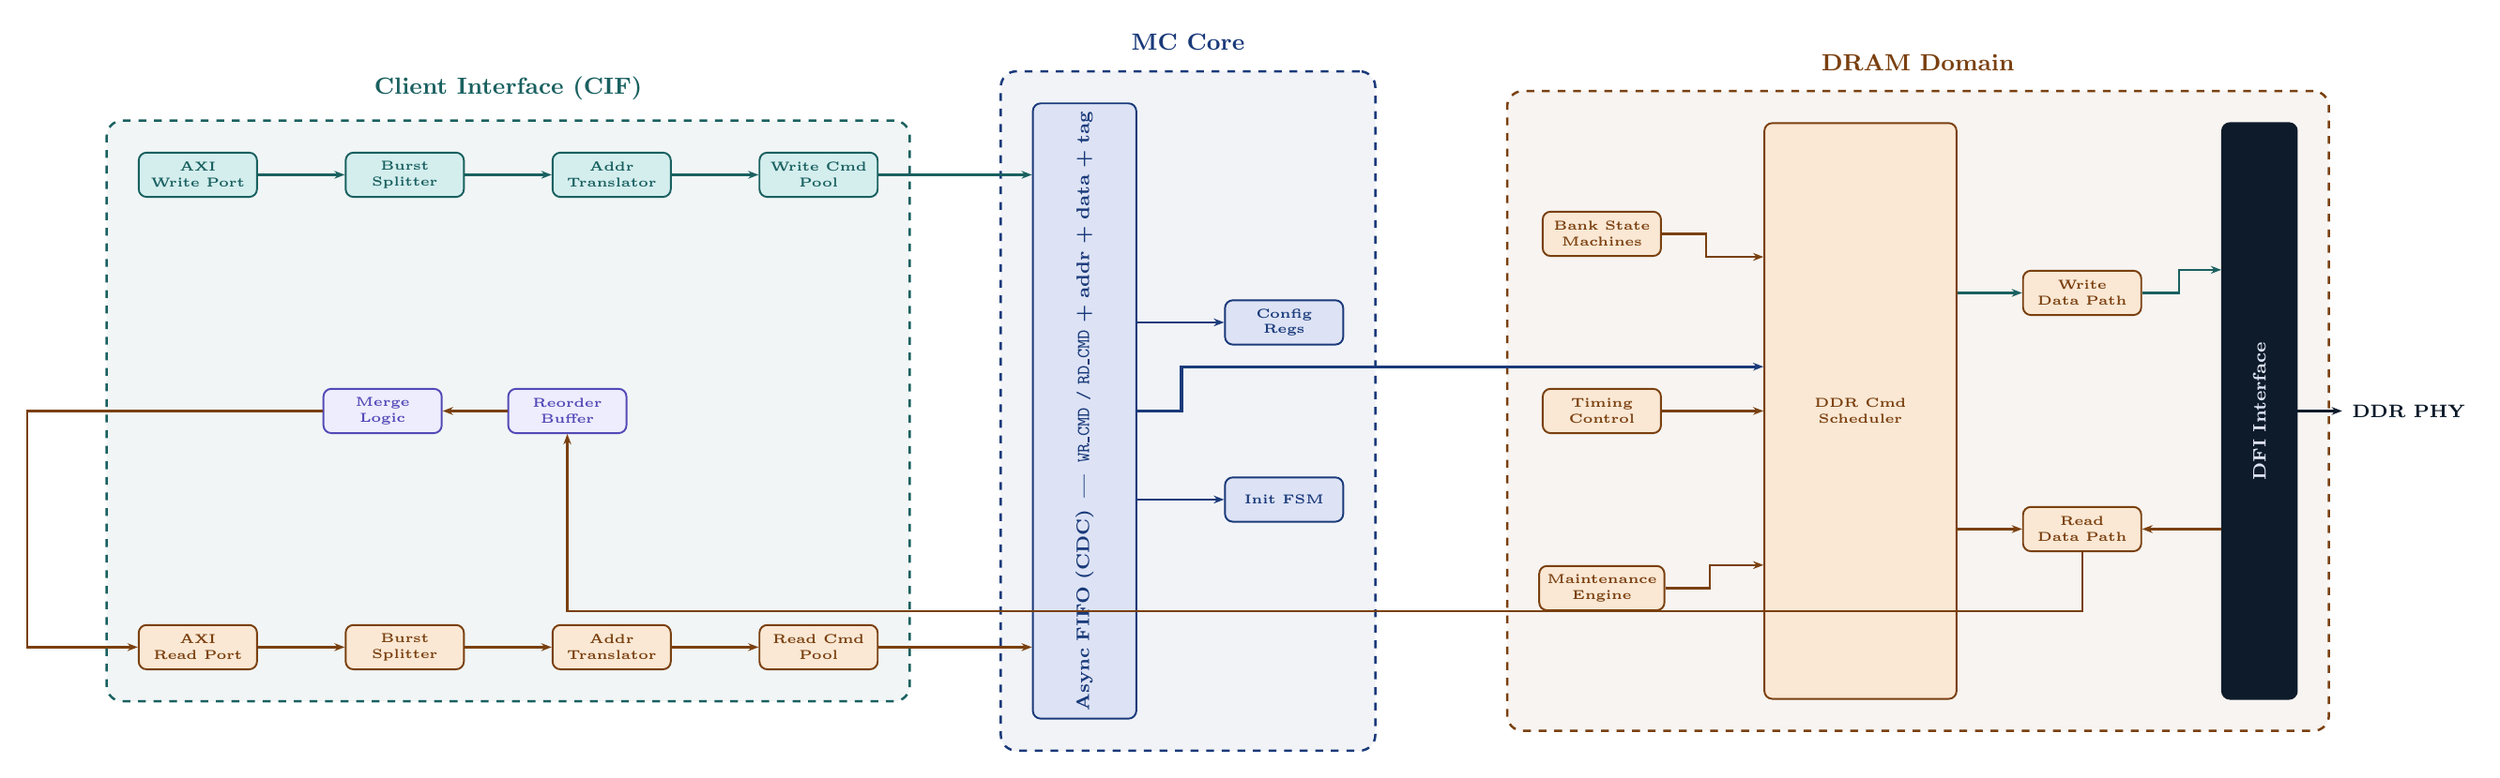
\begin{tikzpicture}[x=1cm,y=1cm]

    \node[sblk=Teal/TealF] (awp) at (-1.5, 3.2) {AXI\\Write Port};
    \node[sblk=Teal/TealF] (bsW) at ( 1.3, 3.2) {Burst\\Splitter};
    \node[sblk=Teal/TealF] (adW) at ( 4.1, 3.2) {Addr\\Translator};
    \node[sblk=Teal/TealF] (wcpl)at ( 6.9, 3.2) {Write Cmd\\Pool};

    \node[sblk=Amber/AmberF](arp) at (-1.5,-3.2) {AXI\\Read Port};
    \node[sblk=Amber/AmberF](bsR) at ( 1.3,-3.2) {Burst\\Splitter};
    \node[sblk=Amber/AmberF](adR) at ( 4.1,-3.2) {Addr\\Translator};
    \node[sblk=Amber/AmberF](rcpl)at ( 6.9,-3.2) {Read Cmd\\Pool};

    \node[sblk=Purp/PurpF] (rrb) at ( 3.5, 0.0) {Reorder\\Buffer};
    \node[sblk=Purp/PurpF] (mlg) at ( 1.0, 0.0) {Merge\\Logic};

    \node[sblk=Blue/BlueF,
          minimum width=1.4cm, minimum height=7.8cm,
          text width=1.1cm] (cdc) at (10.5,0)
          {\rotatebox{90}{\scriptsize Async FIFO (CDC)\enspace|\enspace
            \texttt{WR\_CMD / RD\_CMD} + addr + data + tag}};
    \node[sblk=Blue/BlueF] (cfg)  at (13.2, 1.2) {Config\\Regs};
    \node[sblk=Blue/BlueF] (init) at (13.2,-1.2) {Init FSM};

    \node[sblk=Amber/AmberF] (bfsm)  at (17.5, 2.4) {Bank State\\Machines};
    \node[sblk=Amber/AmberF] (tctl)  at (17.5, 0.0) {Timing\\Control};
    \node[sblk=Amber/AmberF] (maint) at (17.5,-2.4) {Maintenance\\Engine};
    \node[sblk=Amber/AmberF,
          minimum width=2.6cm,minimum height=7.8cm]
                             (sched) at (21.0, 0.0) {DDR Cmd\\Scheduler};
    \node[sblk=Amber/AmberF] (wdp)   at (24.0, 1.6) {Write\\Data Path};
    \node[sblk=Amber/AmberF] (rdp)   at (24.0,-1.6) {Read\\Data Path};
    \node[sblk=Navy/Navy,
          minimum width=1.0cm, minimum height=7.8cm,
          text width=0.8cm] (dfi) at (26.4,0)
          {\color{BlueF}\rotatebox{90}{\scriptsize\bfseries DFI Interface}};

    \begin{scope}[on background layer]
      \node[rgn=Teal,
            fit=(awp)(bsW)(adW)(wcpl)(arp)(bsR)(adR)(rcpl)(rrb)(mlg),
            inner sep=12pt,
            label={[font=\small\bfseries,text=Teal,yshift=4pt]above:Client Interface (CIF)}]
            (cifrgn) {};
      \node[rgn=Blue,
            fit=(cdc)(cfg)(init),
            inner sep=12pt,
            label={[font=\small\bfseries,text=Blue,yshift=4pt]above:MC Core}]
            (mcrgn) {};
      \node[rgn=Amber,
            fit=(bfsm)(tctl)(maint)(sched)(wdp)(rdp)(dfi),
            inner sep=12pt,
            label={[font=\small\bfseries,text=Amber,yshift=4pt]above:DRAM Domain}]
            (dramrgn) {};
    \end{scope}

    \draw[arr=Teal] (awp)--(bsW); \draw[arr=Teal] (bsW)--(adW);
    \draw[arr=Teal] (adW)--(wcpl);
    \draw[arr=Amber](arp)--(bsR); \draw[arr=Amber](bsR)--(adR);
    \draw[arr=Amber](adR)--(rcpl);
    \draw[arr=Teal] (wcpl.east)  -- (cdc.west|-wcpl.east);
    \draw[arr=Amber](rcpl.east)  -- (cdc.west|-rcpl.east);
    \draw[arr=Blue] (cdc.east|-cfg)  -- (cfg.west);
    \draw[arr=Blue] (cdc.east|-init) -- (init.west);
    \draw[arr=Blue,line width=1.2pt]
        (cdc.east|-tctl) -- ++(0.6,0) -- ++(0,0.6) -- (sched.west|-{(0,0.6)});
    \draw[arr=Amber](bfsm.east) --++(0.6,0)|-(sched.west|-bfsm.south);
    \draw[arr=Amber](tctl.east) -- (sched.west);
    \draw[arr=Amber](maint.east)--++(0.6,0)|-(sched.west|-maint.north);
    \draw[arr=Teal] (sched.east|-wdp) -- (wdp.west);
    \draw[arr=Amber](sched.east|-rdp) -- (rdp.west);
    \draw[arr=Teal] (wdp.east)--++(0.5,0)|-(dfi.west|-wdp.north);
    \draw[arr=Amber](dfi.west|-rdp.center) -- (rdp.east);
    \draw[arr=Amber](rdp.south)--++(0,-0.8)-|(rrb.south);
    \draw[arr=Amber](rrb.west)--(mlg.east);
    \draw[arr=Amber](mlg.west)--++(-4.0,0)|-(arp.west);
    \draw[arr=Navy,line width=1.2pt]
        (dfi.east)--++(0.6,0) node[right,font=\scriptsize\bfseries,text=Navy]{DDR PHY};

  \end{tikzpicture}
  }
  \end{center}
  \vspace*{-2pt}
  {\tiny\color{MGray}\textbf{Teal} = CIF\quad
   \textbf{\color{Blue}Blue} = MC Core\quad
   \textbf{\color{Amber}Amber} = DRAM Domain\quad
   $\triangleright$ Today's focus: CIF (slides 4--7) + JEDEC specs (slides 9--11)}
\end{frame}

% ── Slide 4: CIF Zoom ────────────────────────────────────────────────────────
\begin{frame}{Client Interface (CIF) — Zoom In}
              {AXI termination $\rightarrow$ normalized command stream}

  {\scriptsize The CIF terminates the AXI4 subordinate port and converts burst transactions
  into a stream of normalized \texttt{RD\_CMD}/\texttt{WR\_CMD} packets. It has
  \textbf{no knowledge} of DRAM timing, bank state, or refresh.}

  \vspace*{4pt}
  \begin{center}
  \scalebox{0.78}{%
  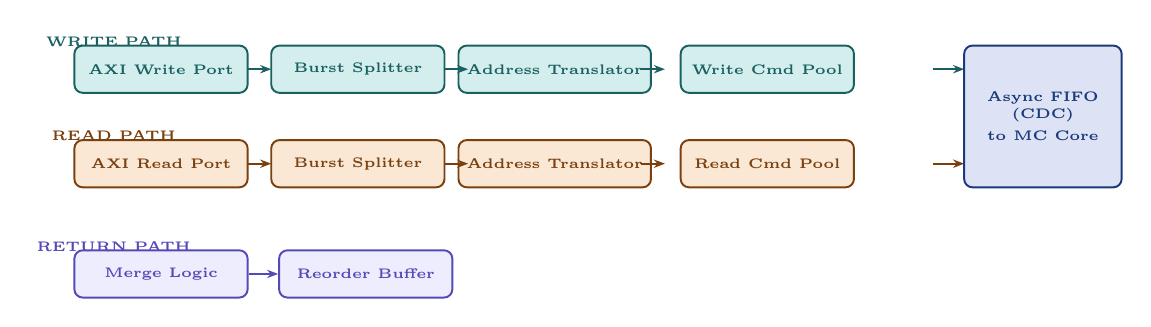
\begin{tikzpicture}[x=1cm,y=1cm]

    \foreach \lbl/\x in {AXI Write Port/0, Burst Splitter/2.5,
                          Address Translator/5.0, Write Cmd Pool/7.7}{
      \node[sblk=Teal/TealF, minimum width=2.2cm] at (\x,1.0) {\lbl};
    }
    \foreach \x in {1.1,3.6,6.1}{
      \draw[arr=Teal] (\x,1.0)--++(0.3,0);
    }
    \node[font=\tiny\bfseries,text=Teal] at (-0.6,1.35) {WRITE PATH};

    \foreach \lbl/\x in {AXI Read Port/0, Burst Splitter/2.5,
                          Address Translator/5.0, Read Cmd Pool/7.7}{
      \node[sblk=Amber/AmberF, minimum width=2.2cm] at (\x,-0.2) {\lbl};
    }
    \foreach \x in {1.1,3.6,6.1}{
      \draw[arr=Amber] (\x,-0.2)--++(0.3,0);
    }
    \node[font=\tiny\bfseries,text=Amber] at (-0.6,0.15) {READ PATH};

    \node[sblk=Blue/BlueF,
          minimum width=2.0cm, minimum height=1.8cm] (cdc) at (11.2,0.4)
          {Async FIFO\\(CDC)\\[2pt]{\tiny to MC Core}};
    \draw[arr=Teal]  (9.8, 1.0) -- (10.2, 1.0);
    \draw[arr=Amber] (9.8,-0.2) -- (10.2,-0.2);

    \node[sblk=Purp/PurpF,minimum width=2.2cm] (ml)  at (0.0,-1.6) {Merge Logic};
    \node[sblk=Purp/PurpF,minimum width=2.2cm] (rob) at (2.6,-1.6) {Reorder Buffer};
    \draw[arr=Purp] (ml)--(rob);
    \node[font=\tiny\bfseries,text=Purp] at (-0.6,-1.25) {RETURN PATH};

  \end{tikzpicture}
  }
  \end{center}

  \vspace*{2pt}
  \begin{columns}[T,totalwidth=\linewidth]
    \scriptsize
    \begin{column}{0.5\linewidth}
      \textbullet\ \textbf{Burst Splitter:} 2-stage — page boundary then BL alignment\\[2pt]
      \textbullet\ \textbf{Addr Translator:} byte addr $\to$ \{rank, bank, row, col\} via reg-file map
    \end{column}
    \begin{column}{0.5\linewidth}
      \textbullet\ \textbf{ROB:} per-AXID HEAD ptr, \{AXID, seqnum\} tag — no cross-ID stall\\[2pt]
      \textbullet\ \textbf{Merge Logic:} fragment buffer + reassembly tracker $\to$ Output Mux
    \end{column}
  \end{columns}
\end{frame}

% ── Slide 5: Burst Splitter ──────────────────────────────────────────────────
\begin{frame}{CIF Block: Burst Splitter}
              {Stage 1 — Page Boundary \quad|\quad Stage 2 — BL Alignment}
  \begin{columns}[T,totalwidth=\linewidth]
    \begin{column}{0.6\linewidth}
    \vspace*{-0.1cm}
    \begin{center}
    \scalebox{0.72}{%
    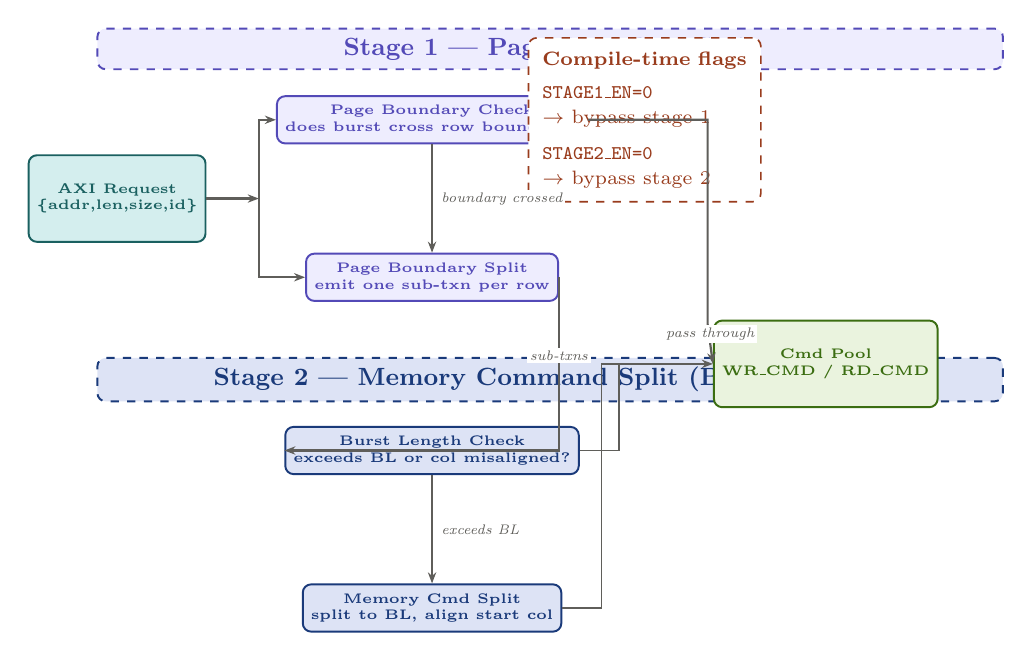
\begin{tikzpicture}[x=1cm,y=1cm]

      \node[rectangle, rounded corners=3pt, draw=Purp, fill=PurpF,
            dashed, line width=0.7pt, font=\small\bfseries, text=Purp,
            minimum width=11.5cm, minimum height=0.45cm] at (6.0,5.1)
            {Stage 1 --- Page Boundary Split};

      \node[sblk=Teal/TealF, minimum width=2.2cm, minimum height=1.1cm]
            (IN) at (0.5,3.2) {AXI Request\\{\tiny\{addr,len,size,id\}}};

      \node[sblk=Purp/PurpF, minimum width=3.2cm] (S1C) at (4.5,4.2)
            {Page Boundary Check\\{\tiny does burst cross row boundary?}};
      \node[sblk=Purp/PurpF, minimum width=3.2cm] (S1S) at (4.5,2.2)
            {Page Boundary Split\\{\tiny emit one sub-txn per row}};

      \node[rectangle, rounded corners=3pt, draw=Blue, fill=BlueF,
            dashed, line width=0.7pt, font=\small\bfseries, text=Blue,
            minimum width=11.5cm, minimum height=0.45cm] at (6.0,0.9)
            {Stage 2 --- Memory Command Split (BL alignment)};

      \node[sblk=Blue/BlueF, minimum width=3.2cm] (S2C) at (4.5,0.0)
            {Burst Length Check\\{\tiny exceeds BL or col misaligned?}};
      \node[sblk=Blue/BlueF, minimum width=3.2cm] (S2S) at (4.5,-2.0)
            {Memory Cmd Split\\{\tiny split to BL, align start col}};

      \node[sblk=Green/GreenF, minimum width=2.2cm, minimum height=1.1cm]
            (OUT) at (9.5,1.1) {Cmd Pool\\{\tiny WR\_CMD / RD\_CMD}};

      \node[rectangle, rounded corners=3pt, draw=BypassR,
            fill=white, line width=0.6pt, dashed,
            font=\fontsize{7}{9}\selectfont, text=BypassR,
            inner sep=5pt, text width=2.6cm] at (7.2,4.2) {%
        \textbf{Compile-time flags}\\[3pt]
        \texttt{STAGE1\_EN=0}\\$\to$ bypass stage 1\\[4pt]
        \texttt{STAGE2\_EN=0}\\$\to$ bypass stage 2
      };

      \coordinate (FORK) at (2.3,3.2);
      \draw[arr=MGray] (IN.east) -- (FORK);
      \draw[arr=MGray] (FORK) |- (S1C.west);
      \draw[arr=MGray] (FORK) |- (S1S.west);
      \draw[arr=MGray] (S1C.south) -- (S1S.north)
            node[lbl,midway,right=2pt]{\tiny boundary crossed};
      \draw[arr=MGray] (S1C.east) -| (8.0,1.6) -- (OUT.west)
            node[lbl,midway,above]{\tiny pass through};
      \draw[arr=MGray] (S1S.east) |- (S2C.west)
            node[lbl,near start,above]{\tiny sub-txns};
      \draw[arr=MGray] (S2C.south) -- (S2S.north)
            node[lbl,midway,right=2pt]{\tiny exceeds BL};
      \coordinate (MERGE) at (7.3,1.1);
      \draw[MGray,line width=0.6pt] (S2C.east)--++(0.5,0)|-(MERGE);
      \draw[MGray,line width=0.6pt] (S2S.east)--++(0.5,0)|-(MERGE);
      \draw[arr=MGray] (MERGE) -- (OUT.west);

    \end{tikzpicture}
    }
    \end{center}
    \end{column}

    \begin{column}{0.38\linewidth}
      \vspace*{0.3cm}
      {\small\bfseries\color{Purp}Stage 1 — Row Boundary}\\[3pt]
      {\scriptsize
      \[
        \text{ROW\_BYTES} = 2^{C} \times \text{BUS\_W\_B}
      \]
      Burst crosses boundary if\\
      $A + \text{LEN\_B} > A_\text{row\_end}$\\[4pt]
      Split: sub-txns confined to one row each.
      }

      \vspace*{8pt}
      {\small\bfseries\color{Blue}Stage 2 — BL Alignment}\\[3pt]
      {\scriptsize
      \[
        \text{CMD\_BYTES} = \text{BL} \times \text{BUS\_W\_B}
      \]
      Unaligned start $\Rightarrow$ partial first cmd\\
      with byte-enable mask \texttt{BE < 0xFF}.\\[4pt]
      Number of cmds:
      \[
        N_\text{cmds} = \Bigl\lceil
          \tfrac{(A' \bmod \text{CMD\_B}) + N_\text{B}}
                {\text{CMD\_B}}
        \Bigr\rceil
      \]
      }

      \vspace*{8pt}
      {\scriptsize\color{BypassR}
      Each stage individually enable/disable\\
      at \textbf{compile time} via\\
      \texttt{STAGE1\_EN} / \texttt{STAGE2\_EN}.
      }
    \end{column}
  \end{columns}
\end{frame}

% ── Slide 6: Address Translator + ROB ────────────────────────────────────────
\begin{frame}{CIF Blocks: Address Translator \& Reorder Buffer}
              {DRAM address mapping · AXI response ordering}

  \begin{columns}[T,totalwidth=\linewidth]
    \begin{column}{0.47\linewidth}
      {\small\bfseries\color{Teal}Address Translator}\\[4pt]

      \begin{center}
      \scalebox{0.78}{%
      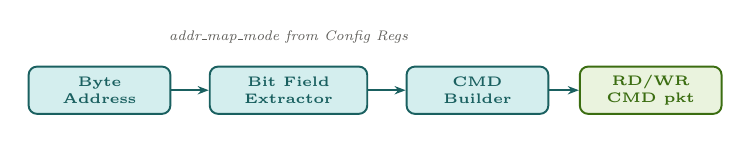
\begin{tikzpicture}[x=1cm,y=1cm]
        \node[sblk=Teal/TealF, minimum width=1.8cm] (ba)  at (0,0) {Byte\\Address};
        \node[sblk=Teal/TealF, minimum width=2.0cm] (bfe) at (2.4,0){Bit Field\\Extractor};
        \node[sblk=Teal/TealF, minimum width=1.8cm] (cb)  at (4.8,0){CMD\\Builder};
        \node[sblk=Green/GreenF,minimum width=1.8cm](out) at (7.0,0){RD/WR\\CMD pkt};
        \draw[arr=Teal](ba)--(bfe); \draw[arr=Teal](bfe)--(cb); \draw[arr=Teal](cb)--(out);
        \node[lbl,above=6pt] at (2.4,0.35) {\tiny addr\_map\_mode from Config Regs};
      \end{tikzpicture}
      }
      \end{center}

      \vspace*{2pt}
      {\scriptsize
      Output tuple: $\{$\texttt{rank, bank\_grp, bank, row, col}$\}$\\[4pt]
      \begin{tabular}{@{}ll@{}}
        \textbf{DDR3} & No bank\_grp field\\
        \textbf{DDR4} & 2 bank\_grp bits added\\
        \textbf{DDR5} & Sub-channel bits in addr\\
      \end{tabular}\\[4pt]
      Bit-field widths are \textbf{register-programmable} — same RTL
      correct for all generations.
      }

      \vspace*{5pt}
      \begin{center}
        \imgplaceholder{0.85\linewidth}{1.8cm}{addr\_translator.png}
      \end{center}
    \end{column}

    \begin{column}{0.51\linewidth}
      {\small\bfseries\color{Purp}Reorder Buffer (ROB)}\\[4pt]

      \begin{center}
      \scalebox{0.78}{%
      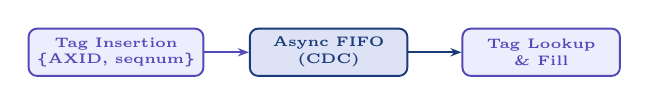
\begin{tikzpicture}[x=1cm,y=1cm]
        \node[sblk=Purp/PurpF,minimum width=2.0cm](ti)  at (0,0)  {Tag Insertion\\{\tiny\{AXID, seqnum\}}};
        \node[sblk=Blue/BlueF, minimum width=2.0cm](cdc) at (2.7,0){Async FIFO\\(CDC)};
        \node[sblk=Purp/PurpF,minimum width=2.0cm](tl)  at (5.4,0){Tag Lookup\\{\tiny \& Fill}};
        \draw[arr=Purp](ti)--(cdc); \draw[arr=Blue](cdc)--(tl);
      \end{tikzpicture}
      }
      \end{center}

      \vspace*{3pt}
      {\scriptsize
      \begin{tabular}{@{}>{\bfseries\color{Purp}}p{3.2cm}
                         @{}>{\color{MGray}}p{4.0cm}@{}}
        \toprule
        Property & Guarantee \\
        \midrule
        Same-AXID ordering
          & Responses retire in strict seqnum order \\[3pt]
        Cross-AXID isolation
          & Per-AXID queues + HEAD ptrs independent \\[3pt]
        Tag uniqueness
          & $\{$AXID, seqnum$\}$ globally unique \\[3pt]
        CDC outside ROB
          & ROB on client clock only \\
        \bottomrule
      \end{tabular}
      }

      \vspace*{4pt}
      \begin{center}
        \imgplaceholder{0.85\linewidth}{1.8cm}{rob.png}
      \end{center}
    \end{column}
  \end{columns}
\end{frame}

% ── Slide 7: Merge Logic ─────────────────────────────────────────────────────
\begin{frame}{CIF Block: Merge Logic}
              {Fragment reassembly after DRAM-domain reordering}

  {\scriptsize When the Burst Splitter splits a single AXI read into multiple
  sub-commands, each may return out of order from the DRAM scheduler.
  Merge Logic collects all fragments and concatenates them in the correct order
  before the ROB.}

  \vspace*{4pt}

  \begin{center}
  \scalebox{0.80}{%
  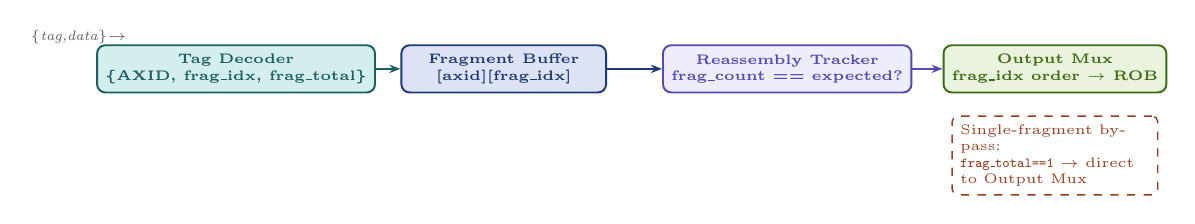
\begin{tikzpicture}[x=1cm,y=1cm]
    \node[lbl] at (-1.2,0.4) {\{tag,data\}$\to$};
    \node[sblk=Teal/TealF,  minimum width=2.6cm] (td)  at ( 0.8, 0)
          {Tag Decoder\\{\tiny\{AXID, frag\_idx, frag\_total\}}};
    \node[sblk=Blue/BlueF,  minimum width=2.6cm] (fb)  at ( 4.2, 0)
          {Fragment Buffer\\{\tiny [axid][frag\_idx]}};
    \node[sblk=Purp/PurpF,  minimum width=2.8cm] (rt)  at ( 7.8, 0)
          {Reassembly Tracker\\{\tiny frag\_count == expected?}};
    \node[sblk=Green/GreenF,minimum width=2.6cm] (om)  at (11.2, 0)
          {Output Mux\\{\tiny frag\_idx order $\to$ ROB}};
    \draw[arr=Teal] (td)--(fb);
    \draw[arr=Blue] (fb)--(rt);
    \draw[arr=Purp] (rt)--(om);
    \node[rectangle, rounded corners=2pt, draw=BypassR, fill=white,
          dashed, line width=0.5pt, font=\tiny, text=BypassR,
          inner sep=3pt, text width=2.4cm] at (11.2,-1.1)
          {Single-fragment bypass:\\\texttt{frag\_total==1} $\to$ direct to Output Mux};
  \end{tikzpicture}
  }
  \end{center}

  \vspace*{4pt}

  \begin{columns}[T,totalwidth=\linewidth]
    \begin{column}{0.245\linewidth}
      \infocard{Teal}{TealF}{%
        {\tiny\bfseries\color{Teal}Tag Decoder}\\[2pt]
        {\tiny Receives each \{tag,data\} beat. Extracts
        AXID, cmd ID, \texttt{frag\_idx}, \texttt{frag\_total} from tag field.}
      }
    \end{column}
    \begin{column}{0.245\linewidth}
      \infocard{Blue}{BlueF}{%
        {\tiny\bfseries\color{Blue}Fragment Buffer}\\[2pt]
        {\tiny Stores data at \texttt{[axid][frag\_idx]}. Slot: data word + valid bit.
        Non-sequential writes OK.}
      }
    \end{column}
    \begin{column}{0.245\linewidth}
      \infocard{Purp}{PurpF}{%
        {\tiny\bfseries\color{Purp}Reassembly Tracker}\\[2pt]
        {\tiny Per-AXID: \texttt{frag\_count} (arrived), \texttt{expected}
        (from \texttt{frag\_total} on first fragment).}
      }
    \end{column}
    \begin{column}{0.245\linewidth}
      \infocard{Green}{GreenF}{%
        {\tiny\bfseries\color{Green}Output Mux}\\[2pt]
        {\tiny Reads slots \texttt{0..frag\_total$-$1} in order, concatenates
        into full burst, forwards to ROB.}
      }
    \end{column}
  \end{columns}

  \vspace*{4pt}
  \begin{center}
    \imgplaceholder{0.7\linewidth}{1.4cm}{merge\_logic.png}
  \end{center}
\end{frame}

% ── Slide 8: JEDEC Comparison Table ──────────────────────────────────────────
\begin{frame}{DDR3 / DDR4 / DDR5 — JEDEC Key Specs}
              {JESD79-3 · JESD79-4 · JESD79-5}

  \vspace*{-0.1cm}
  \begin{center}
  {\scriptsize
  \renewcommand{\arraystretch}{1.18}
  \begin{tabular}{%
    >{\bfseries\color{Navy}}p{2.8cm}
    >{\color{MGray}}p{2.85cm}
    >{\color{MGray}}p{2.85cm}
    >{\color{MGray}}p{3.1cm}}

  \rowcolor{Navy}
  \multicolumn{1}{>{\bfseries\color{white}}p{2.8cm}}{Parameter}
  & \multicolumn{1}{>{\bfseries\color{white}}p{2.85cm}}{\cellcolor{ddr3col}DDR3}
  & \multicolumn{1}{>{\bfseries\color{white}}p{2.85cm}}{\cellcolor{ddr4col}DDR4}
  & \multicolumn{1}{>{\bfseries\color{white}}p{3.1cm}}{\cellcolor{ddr5col}DDR5}
  \\

  \rowcolor{LGray!50}
  Standard          & JESD79-3F             & JESD79-4C             & JESD79-5B             \\
  Data Rate (MT/s)  & 800\,--\,2133         & 1600\,--\,3200        & 3200\,--\,6400+       \\
  \rowcolor{LGray!50}
  Prefetch          & 8n                    & 8n                    & 16n (BL16)            \\
  Burst Length (BL) & BL8 (fixed/fly)       & BL8 (fixed/fly)       & BL16 mandatory        \\
  \rowcolor{LGray!50}
  Bank Groups       & None                  & 2 / 4 BGs             & 8 BGs (sub-ch.)       \\
  Channels          & Single                & Single                & Sub-channel ($\times$2) \\
  \rowcolor{LGray!50}
  IO Voltage        & 1.5\,V / 1.35\,V      & 1.2\,V                & 1.1\,V                \\
  On-Die ECC        & Optional              & Optional              & Required ($\times$4 org) \\
  \rowcolor{LGray!50}
  Refresh           & tREFI = 7.8\,\textmu s & tREFI = 7.8\,\textmu s & Dual-rate refresh    \\
  Termination       & RTT\_NOM              & RTT\_PARK added        & RTT\_PARK + DFITMG   \\
  \rowcolor{LGray!50}
  Key timing params & tRCD, tRP, tRAS, tWR, tRFC
                    & tWTR\_L/S added       & tRFC1/2/sb, tCS       \\
  \end{tabular}
  }
  \end{center}

  \vspace*{3pt}
  \begin{center}
    \imgplaceholder{0.65\linewidth}{1.5cm}{jedec\_tRCD\_tRAS\_tRP.png}
  \end{center}
\end{frame}

% ── Slide 9: DDR3 JEDEC Deep-Dive ────────────────────────────────────────────
\begin{frame}{DDR3 JEDEC Deep-Dive}
              {JESD79-3F · Key Timing · Init Sequence · MRS}

  \begin{columns}[T,totalwidth=\linewidth]

    \begin{column}{0.50\linewidth}
      \infocard{ddr3col}{BlueF!60!white}{%
        {\small\bfseries\color{ddr3col}Critical Timing Parameters}\\[4pt]
        \scriptsize
        \begin{tabular}{@{}>{\bfseries}l@{\hspace{6pt}}l@{}}
          tRCD & RAS-to-CAS delay; row open to col cmd \\
          tRP  & Row precharge time; min between PRE and ACT \\
          tRAS & Min row active time (tRCD + tRTP) \\
          tRC  & Row cycle time = tRAS + tRP \\
          tWR  & Write recovery; data valid after WR before PRE \\
          tRFC & Refresh cycle time; scales with density \\
          tFAW & 4-bank activation window; max 4 ACT in tFAW \\
          tWTR & Write-to-read turnaround; bus direction switch \\
          CL   & CAS latency; clocks from RD cmd to first data \\
        \end{tabular}
      }

      \vspace*{5pt}
      \infocard{Purp}{PurpF}{%
        {\small\bfseries\color{Purp}Mode Register Set (MRS)}\\[4pt]
        \scriptsize
        \textbullet\ MR0: CL, BL, DLL reset, write recovery, read DQS \\[2pt]
        \textbullet\ MR1: DLL enable, drive strength, RTT\_NOM, AL \\[2pt]
        \textbullet\ MR2: CWL, ASR, SRT, RTT\_WR \\[2pt]
        \textbullet\ MR3: MPR (Multi-Purpose Register) for read training
      }
    \end{column}

    \begin{column}{0.48\linewidth}
      \infocard{Amber}{AmberF}{%
        {\small\bfseries\color{Amber}DDR3 Initialization Sequence}\\[4pt]
        \scriptsize
        \begin{enumerate}\setlength\itemsep{2pt}
          \item Apply stable V\textsubscript{DD}, V\textsubscript{DDSPD} — min 200\,\textmu s
          \item Assert \texttt{RESET\#} low $\ge$\,200\,\textmu s
          \item De-assert \texttt{RESET\#}; CKE low $\ge$\,500\,\textmu s
          \item Apply stable CK; bring CKE high after t\textsubscript{XSDLL}
          \item Issue NOP $\ge$\,t\textsubscript{XPR} clocks
          \item Load MR2 $\to$ MR3 $\to$ MR1 $\to$ MR0 (this order)
          \item Issue ZQCL (ZQ calibration long) — 512 clocks
          \item DRAM ready for normal operation
        \end{enumerate}
      }

      \vspace*{5pt}
      \begin{center}
        \imgplaceholder{\linewidth}{2.8cm}{ddr3\_init\_waveform.png}
      \end{center}
    \end{column}

  \end{columns}
\end{frame}

% ── Slide 10: DDR4 JEDEC Deep-Dive ───────────────────────────────────────────
\begin{frame}{DDR4 JEDEC Deep-Dive}
              {JESD79-4C · Bank Groups · tWTR\_L/S · Write Levelling}

  \begin{columns}[T,totalwidth=\linewidth]

    \begin{column}{0.50\linewidth}
      \infocard{ddr4col}{GreenF!60!white}{%
        {\small\bfseries\color{ddr4col}Bank Group Architecture}\\[4pt]
        \scriptsize
        \textbullet\ DDR4: 2 or 4 bank groups (BG), 4 banks each\\[2pt]
        \textbullet\ Intra-BG turnaround (same BG, diff bank): slower — must respect t\textsubscript{RRD\_L}, t\textsubscript{WTR\_L}\\[2pt]
        \textbullet\ Inter-BG turnaround (diff BG): faster — t\textsubscript{RRD\_S}, t\textsubscript{WTR\_S}\\[2pt]
        \textbullet\ Scheduler exploits BG interleaving for near-zero bus-turnaround penalty\\[2pt]
        \textbullet\ Address bit A17/BG1 selects bank group; decoded in addr translator
      }

      \vspace*{5pt}
      \infocard{Blue}{BlueF}{%
        {\small\bfseries\color{Blue}New Timing Parameters vs DDR3}\\[4pt]
        \scriptsize
        \begin{tabular}{@{}>{\bfseries}l@{\hspace{6pt}}p{5.4cm}@{}}
          tWTR\_L & Write-to-read, same bank group — longer \\
          tWTR\_S & Write-to-read, different bank group — shorter \\
          tRRD\_L & ACT-to-ACT same BG \\
          tRRD\_S & ACT-to-ACT different BG \\
          tCCD\_L & CAS-to-CAS same BG \\
          tCCD\_S & CAS-to-CAS different BG \\
        \end{tabular}
      }
    \end{column}

    \begin{column}{0.48\linewidth}
      \infocard{Amber}{AmberF}{%
        {\small\bfseries\color{Amber}PHY Training Procedures (DDR4)}\\[4pt]
        \scriptsize
        \begin{enumerate}\setlength\itemsep{2pt}
          \item \textbf{Write Levelling:} DQS launched; DRAM echoes
                on rising edge of CK — adjusts DQS-to-CK skew per lane
          \item \textbf{Read Gate Training:} PHY determines preamble
                window; gates DQS capture
          \item \textbf{Read Centering:} Sweeps VREF on DQ bus to find
                centre of eye
          \item \textbf{Write Centering:} PHY DQ delay tuned vs DQS
          \item \textbf{ZQ Calibration:} Periodically issues ZQCS;
                updates R\textsubscript{ZQ} impedance code
        \end{enumerate}
      }

      \vspace*{5pt}
      \begin{center}
        \imgplaceholder{\linewidth}{2.8cm}{ddr4\_bankgroup\_timing.png}
      \end{center}
    \end{column}

  \end{columns}
\end{frame}

% ── Slide 11: DDR5 JEDEC Deep-Dive ───────────────────────────────────────────
\begin{frame}{DDR5 JEDEC Deep-Dive}
              {JESD79-5B · BL16 · Sub-channel · On-Die ECC · Dual Refresh}

  \begin{columns}[T,totalwidth=\linewidth]

    \begin{column}{0.50\linewidth}
      \infocard{ddr5col}{PurpF!50!white}{%
        {\small\bfseries\color{ddr5col}Architectural Changes vs DDR4}\\[4pt]
        \scriptsize
        \textbullet\ \textbf{BL16 mandatory:} 16n prefetch; burst is 64\,B per sub-channel\\[2pt]
        \textbullet\ \textbf{Sub-channels:} One DIMM $=$ two independent 32-bit sub-channels
                (SA/SB); MC treats each as separate rank\\[2pt]
        \textbullet\ \textbf{On-Die ECC:} Required for $\times$4 org; corrects single-bit errors
                before data leaves DRAM die — transparent to MC\\[2pt]
        \textbullet\ \textbf{8 Bank Groups:} 32 banks per sub-channel; 2$\times$ parallelism vs DDR4\\[2pt]
        \textbullet\ \textbf{1.1\,V V\textsubscript{DD}:} Lower swing; VDDQ separate from VDD\\[2pt]
        \textbullet\ \textbf{CA bus:} Command/Address bus width doubled; parity added
      }

      \vspace*{5pt}
      \infocard{Teal}{TealF}{%
        {\small\bfseries\color{Teal}Dual-Rate Refresh (DDR5)}\\[4pt]
        \scriptsize
        \textbullet\ \textbf{Normal rate:} tREFI = 3.9\,\textmu s (2$\times$ faster than DDR4)\\[2pt]
        \textbullet\ \textbf{Fine granularity:} Per-bank refresh (PBR) — refresh individual
                banks, not all; reduces refresh penalty\\[2pt]
        \textbullet\ \textbf{tRFC1 / tRFC2:} Two refresh modes — tRFC2 shorter, uses
                2$\times$ refresh rate (high-temp operation)\\[2pt]
        \textbullet\ \textbf{Alert mechanism:} DRAM signals MC via \texttt{ALERT\_n} if
                refresh deferrals exceed limit
      }
    \end{column}

    \begin{column}{0.48\linewidth}
      \infocard{Amber}{AmberF}{%
        {\small\bfseries\color{Amber}DDR5 Init \& Training Additions}\\[4pt]
        \scriptsize
        \begin{enumerate}\setlength\itemsep{2pt}
          \item \textbf{BCOM training:} Sideband command bus training
                before main CA bus functional
          \item \textbf{PDA mode:} Per-DRAM addressability — tune MRS
                per individual DRAM device on bus
          \item \textbf{2$\times$ MRS sets:} Extended mode register space;
                additional latency + ODT configs
          \item \textbf{RTT\_PARK + DFITMG:} Runtime-switchable ODT;
                MC signals via DFI timing parameters
          \item \textbf{CA parity:} Odd parity on CA bus; DRAM latches
                and validates each command frame
        \end{enumerate}
      }

      \vspace*{5pt}
      \begin{center}
        \imgplaceholder{\linewidth}{2.2cm}{ddr5\_subchannel\_arch.png}
      \end{center}

      \vspace*{3pt}
      \begin{center}
        \imgplaceholder{\linewidth}{1.8cm}{ddr5\_refresh\_timeline.png}
      \end{center}
    \end{column}

  \end{columns}
\end{frame}

\end{document}
